\ifx\wholebook\relax\else

% --------------------------------------------
% Lulu:

    \documentclass[a4paper,12pt,twoside]{../includes/ThesisStyle}

	\usepackage[T1]{fontenc} %%%key to get copy and paste for the code!
%\usepackage[utf8]{inputenc} %%% to support copy and paste with accents for frnehc stuff
\usepackage{times}
\usepackage{ifthen}
\usepackage{xspace}
\usepackage{alltt}
\usepackage{latexsym}
\usepackage{url}            
\usepackage{amssymb}
\usepackage{amsfonts}
\usepackage{amsmath}
\usepackage{stmaryrd}
\usepackage{enumerate}
\usepackage{cite}
%\usepackage[pdftex,colorlinks=true,pdfstartview=FitV,linkcolor=blue,citecolor=blue,urlcolor=blue]{hyperref}
\usepackage{xspace}
%\usepackage{graphicx}
\usepackage{subfigure}
\usepackage[scaled=0.85]{helvet}
        
        
\newcommand{\sepe}{\mbox{>>}}
\newcommand{\pack}[1]{\emph{#1}}
\newcommand{\ozo}{\textsc{oZone}\xspace}
\newcommand\currentissues{\par\smallskip\textbf{Current Issues -- }}

\newboolean{showcomments}
\setboolean{showcomments}{true}
\ifthenelse{\boolean{showcomments}}
  {\newcommand{\bnote}[2]{
	\fbox{\bfseries\sffamily\scriptsize#1}
    {\sf\small$\blacktriangleright$\textit{#2}$\blacktriangleleft$}
    % \marginpar{\fbox{\bfseries\sffamily#1}}
   }
   \newcommand{\cvsversion}{\emph{\scriptsize$-$Id: macros.tex,v 1.1.1.1 2007/02/28 13:43:36 bergel Exp $-$}}
  }
  {\newcommand{\bnote}[2]{}
   \newcommand{\cvsversion}{}
  } 


\newcommand{\here}{\bnote{***}{CONTINUE HERE}}
\newcommand{\nb}[1]{\bnote{NB}{#1}}
\newcommand{\fix}[1]{\bnote{FIX}{#1}}
%%%% add your own macros 

\newcommand{\sd}[1]{\bnote{Stef}{#1}}
\newcommand{\ja}[1]{\bnote{Jannik}{#1}}
\newcommand{\na}[1]{\bnote{Nico}{#1}}
%%% 


\newcommand{\figref}[1]{Figure~\ref{fig:#1}}
\newcommand{\figlabel}[1]{\label{fig:#1}}
\newcommand{\tabref}[1]{Table~\ref{tab:#1}}
\newcommand{\layout}[1]{#1}
\newcommand{\commented}[1]{}
\newcommand{\secref}[1]{Section \ref{sec:#1}}
\newcommand{\seclabel}[1]{\label{sec:#1}}

%\newcommand{\ct}[1]{\textsf{#1}}
\newcommand{\stCode}[1]{\textsf{#1}}
\newcommand{\stMethod}[1]{\textsf{#1}}
\newcommand{\sep}{\texttt{>>}\xspace}
\newcommand{\stAssoc}{\texttt{->}\xspace}

\newcommand{\stBar}{$\mid$}
\newcommand{\stSelector}{$\gg$}
\newcommand{\ret}{\^{}}
\newcommand{\msup}{$>$}
%\newcommand{\ret}{$\uparrow$\xspace}

\newcommand{\myparagraph}[1]{\noindent\textbf{#1.}}
\newcommand{\eg}{\emph{e.g.,}\xspace}
\newcommand{\ie}{\emph{i.e.,}\xspace}
\newcommand{\ct}[1]{{\textsf{#1}}\xspace}


\newenvironment{code}
    {\begin{alltt}\sffamily}
    {\end{alltt}\normalsize}

\newcommand{\defaultScale}{0.55}
\newcommand{\pic}[3]{
   \begin{figure}[h]
   \begin{center}
   \includegraphics[scale=\defaultScale]{#1}
   \caption{#2}
   \label{#3}
   \end{center}
   \end{figure}
}

\newcommand{\twocolumnpic}[3]{
   \begin{figure*}[!ht]
   \begin{center}
   \includegraphics[scale=\defaultScale]{#1}
   \caption{#2}
   \label{#3}
   \end{center}
   \end{figure*}}

\newcommand{\infe}{$<$}
\newcommand{\supe}{$\rightarrow$\xspace}
\newcommand{\di}{$\gg$\xspace}
\newcommand{\adhoc}{\textit{ad-hoc}\xspace}

\usepackage{url}            
\makeatletter
\def\url@leostyle{%
  \@ifundefined{selectfont}{\def\UrlFont{\sf}}{\def\UrlFont{\small\sffamily}}}
\makeatother
% Now actually use the newly defined style.
\urlstyle{leo}



	\usepackage{amsmath,amssymb}             % AMS Math
% \usepackage[french]{babel}
\usepackage[latin1]{inputenc}
\usepackage[T1]{fontenc}
\usepackage[left=1.5in,right=1.3in,top=1.1in,bottom=1.1in,includefoot,includehead,headheight=13.6pt]{geometry}
\renewcommand{\baselinestretch}{1.05}

\usepackage{multicol}

% Table of contents for each chapter

\usepackage[nottoc, notlof, notlot]{tocbibind}
\usepackage{minitoc}
\setcounter{minitocdepth}{1}
\mtcindent=15pt
% Use \minitoc where to put a table of contents

\usepackage{enumitem}

\usepackage{aecompl}

% Glossary / list of abbreviations

%\usepackage[intoc]{nomencl}
%\renewcommand{\nomname}{List of Abbreviations}
%
%\makenomenclature

% My pdf code

\usepackage[pdftex]{graphicx}
\usepackage[a4paper,pagebackref,hyperindex=true]{hyperref}

\usepackage{pgfplotstable,booktabs,colortbl}
\pgfplotsset{compat=1.8}

% Links in pdf
\usepackage{color}
\definecolor{linkcol}{rgb}{0,0,0.4} 
\definecolor{citecol}{rgb}{0.5,0,0} 

% Change this to change the informations included in the pdf file

% See hyperref documentation for information on those parameters

\hypersetup
{
bookmarksopen=true,
pdftitle="Sista: a Metacircular Architecture for Runtime Optimisation Persistence",
pdfauthor="Clement BERA", 
pdfsubject="Thesis", %subject of the document
%pdftoolbar=false, % toolbar hidden
pdfmenubar=true, %menubar shown
pdfhighlight=/O, %effect of clicking on a link
colorlinks=true, %couleurs sur les liens hypertextes
pdfpagemode=None, %aucun mode de page
pdfpagelayout=SinglePage, %ouverture en simple page
pdffitwindow=true, %pages ouvertes entierement dans toute la fenetre
linkcolor=linkcol, %couleur des liens hypertextes internes
citecolor=citecol, %couleur des liens pour les citations
urlcolor=linkcol %couleur des liens pour les url
}

% definitions.
% -------------------

\setcounter{secnumdepth}{3}
\setcounter{tocdepth}{1}

% Some useful commands and shortcut for maths:  partial derivative and stuff

\newcommand{\pd}[2]{\frac{\partial #1}{\partial #2}}
\def\abs{\operatorname{abs}}
\def\argmax{\operatornamewithlimits{arg\,max}}
\def\argmin{\operatornamewithlimits{arg\,min}}
\def\diag{\operatorname{Diag}}
\newcommand{\eqRef}[1]{(\ref{#1})}

\usepackage{rotating}                    % Sideways of figures & tables
%\usepackage{bibunits}
%\usepackage[sectionbib]{chapterbib}          % Cross-reference package (Natural BiB)
%\usepackage{natbib}                  % Put References at the end of each chapter
                                         % Do not put 'sectionbib' option here.
                                         % Sectionbib option in 'natbib' will do.
\usepackage{fancyhdr}                    % Fancy Header and Footer

% \usepackage{txfonts}                     % Public Times New Roman text & math font
  
%%% Fancy Header %%%%%%%%%%%%%%%%%%%%%%%%%%%%%%%%%%%%%%%%%%%%%%%%%%%%%%%%%%%%%%%%%%
% Fancy Header Style Options

\pagestyle{fancy}                       % Sets fancy header and footer
\fancyfoot{}                            % Delete current footer settings

%\renewcommand{\chaptermark}[1]{         % Lower Case Chapter marker style
%  \markboth{\chaptername\ \thechapter.\ #1}}{}} %

%\renewcommand{\sectionmark}[1]{         % Lower case Section marker style
%  \markright{\thesection.\ #1}}         %

\fancyhead[LE,RO]{\bfseries\thepage}    % Page number (boldface) in left on even
% pages and right on odd pages
\fancyhead[RE]{\bfseries\nouppercase{\leftmark}}      % Chapter in the right on even pages
\fancyhead[LO]{\bfseries\nouppercase{\rightmark}}     % Section in the left on odd pages

\let\headruleORIG\headrule
\renewcommand{\headrule}{\color{black} \headruleORIG}
\renewcommand{\headrulewidth}{1.0pt}
\usepackage{colortbl}
\arrayrulecolor{black}

\fancypagestyle{plain}{
  \fancyhead{}
  \fancyfoot{}
  \renewcommand{\headrulewidth}{0pt}
}

\usepackage{algorithm}
\usepackage[noend]{algorithmic}

%%% Clear Header %%%%%%%%%%%%%%%%%%%%%%%%%%%%%%%%%%%%%%%%%%%%%%%%%%%%%%%%%%%%%%%%%%
% Clear Header Style on the Last Empty Odd pages
\makeatletter

\def\cleardoublepage{\clearpage\if@twoside \ifodd\c@page\else%
  \hbox{}%
  \thispagestyle{empty}%              % Empty header styles
  \newpage%
  \if@twocolumn\hbox{}\newpage\fi\fi\fi}

\makeatother
 
%%%%%%%%%%%%%%%%%%%%%%%%%%%%%%%%%%%%%%%%%%%%%%%%%%%%%%%%%%%%%%%%%%%%%%%%%%%%%%% 
% Prints your review date and 'Draft Version' (From Josullvn, CS, CMU)
\newcommand{\reviewtimetoday}[2]{\special{!userdict begin
    /bop-hook{gsave 20 710 translate 45 rotate 0.8 setgray
      /Times-Roman findfont 12 scalefont setfont 0 0   moveto (#1) show
      0 -12 moveto (#2) show grestore}def end}}
% You can turn on or off this option.
% \reviewtimetoday{\today}{Draft Version}
%%%%%%%%%%%%%%%%%%%%%%%%%%%%%%%%%%%%%%%%%%%%%%%%%%%%%%%%%%%%%%%%%%%%%%%%%%%%%%% 

\newenvironment{maxime}[1]
{
\vspace*{0cm}
\hfill
\begin{minipage}{0.5\textwidth}%
%\rule[0.5ex]{\textwidth}{0.1mm}\\%
\hrulefill $\:$ {\bf #1}\\
%\vspace*{-0.25cm}
\it 
}%
{%

\hrulefill
\vspace*{0.5cm}%
\end{minipage}
}

\let\minitocORIG\minitoc
\renewcommand{\minitoc}{\minitocORIG \vspace{1.5em}}

\usepackage{multirow}
\usepackage{slashbox}

\newenvironment{bulletList}%
{ \begin{list}%
	{$\bullet$}%
	{\setlength{\labelwidth}{25pt}%
	 \setlength{\leftmargin}{30pt}%
	 \setlength{\itemsep}{\parsep}}}%
{ \end{list} }

\newtheorem{definition}{D�finition}
\renewcommand{\epsilon}{\varepsilon}

% centered page environment

\newenvironment{vcenterpage}
{\newpage\vspace*{\fill}\thispagestyle{empty}\renewcommand{\headrulewidth}{0pt}}
{\vspace*{\fill}}



	\graphicspath{{.}{../figures/}}
	\begin{document}
\fi

\chapter{Existing Pharo runtime}
\label{chap:existing}
\minitoc

%global intro
This chapter describes the Smalltalk dialect Pharo and part of its implementation. The Sista architecture was originally designed to improve the performance of the Pharo VM by adding speculative optimisations. Some existing features and implementation details already present in Pharo impacted several design decisions. They are detailled in this chapter to help the reader understanding the design decisions explained in further chapters. The chapter is not meant to explain the whole existing implementation, but only the most relevant points for the thesis. 

Pharo is an object-oriented language. Everything is an object, including classes or bytecoded versions of methods. It is dynamically-typed and every call is a virtual call. The virtual machine relies on a bytecode interpreter and a baseline JIT to gain performance. Modern Smalltalks directly inherit from Smalltalk-80~\cite{Gold83a} but have evolved during the past 35 years. For example, real closures and exceptions were added.

The chapter successively describes the Pharo programming language, the interface with its VM and some aspects of the VM implementation.

\section{Pharo programming language}

This section details three main aspects of the programming language: native thread management, stack frame reification and snapshots.

\paragraph{Native threads management.}

Pharo features a global interpreter lock, similarly to python. Only calls to external libraries through the foreign function interface and specific virtual machine extensions have access to the other native threads. All the different virtual machine tasks, such as bytecode interpretation, machine code execution, just-in-time compilation or garbage collection are not done concurrently. This has a impact on design decisions because several other VMs implement the optimising JIT in concurrent native threads to the application (CITE). As Scorch is written in Pharo, the optimisation of v-functions and the application optimised are running in the same native thread.

%TODO, closures and NLR?

\paragraph{Stack frame reification.}

The current VM evolved from the VM specified in the blue book~\cite{Gold83a}. The original specification relied on a spaghetti stack: the execution stack was represented as a linked list of v-function activations. Each v-function activation was represented as an object that could be read or written by the program. Over the years, Deutsch and Schiffman~\cite{Deut84a} changed the representation of the stack in the VM to use an execution stack similar to the one used in other programming languages, where stack frames are next to each other on a single stack. However, the VM still provides the ability to the programmer to read and write reified stack frames as if they where objects. To do so, each stack frame is reified as an object on demand. 

The reification of a stack frame abstracts away from the low-level details, a reified stack frame accessed from the language always looks like it is a v-function activation. A reified frame is exactly the same if the VM is started with the interpreter only or with the hybrid interpreter plus baseline JIT runtime. Conceptually, for the Smalltalk developer, Smalltalk code is interpreted and the reified frame always look like so. In fact, it is possible that some developers manipulate the stack without even knowing that there are n-frame or v-frame in practice in the VM.

The reification of the stack frames is used in three main places: the debugger, exceptions and continuations. For the two latter, they are implemented in Smalltalk on top of the stack frame reification, without any special VM support. In the Sista architecture, as Scorch is written in Pharo, it can use this feature to instrospect or modify the stack.

\paragraph{Snapshots.}

A snapshot~\footnote{Smalltalk developers use the term \emph{image} instead of snapshot.} is a sequence of bytes that represents a serialized form of all the objects present at a precise moment in the runtime. As everything is an object in Smalltalk, including green threads, the virtual machine can, at start-up, load all the objects from a snapshot and resume the execution based on the active green thread precised by the snapshot. In fact, this is the normal way of launching a Smalltalk runtime. 

One interesting problem in snapshots is how to save the execution stack, \ie the green threads. It possible in the existing VM to convert reify each stack frame into an object. To perform a snapshot, each stack frame is reified and only objects are saved in the snapshot. When the snapshot is restarted, the VM recreates a stack frame for each reified frame lazily. As discussed in the previous paragraph, all reified frames are in virtual state. In any case, snapshots cannot save n-frames because they are platform-independent. In the Pharo VM for example, a snapshot can be taken on a laptop using a x86 processor and restarted on a raspberry pie using a ARMv6 processor.

%%%%%%%%%%%%%%%%%%%%%%%%%%%%%%%%%%%%%%%%%%%%%%%%%%%%%%%%%%%%%%%%%%%%%%%%%%%%%%%%%%%%%%%%%%%%%%%%%%%%%%%%%%%%%%%%%%%%%%%%%%%%%%%

\section{Language-VM interface}

Pharo interfaces with its VM in two different ways:
\begin{enumerate}
	\item Pharo can instantiate v-functions and install them so the VM can execute them.
	\item A small list of objects is registered in the VM so the VM can access them directly.
\end{enumerate}

\paragraph{Virtual function representation.}

As everything is an object in Pharo, virtual functions are objects. A v-function is composed of a function's header, a list of literals, a list of bytecodes and a reference to its source code as shown on figure \ref{fig:CompiledCode}. The function's header contains information required for the function's execution such as the number of temporary variables or the size of the frame required.

\begin{figure}[h!]
    \begin{center}
        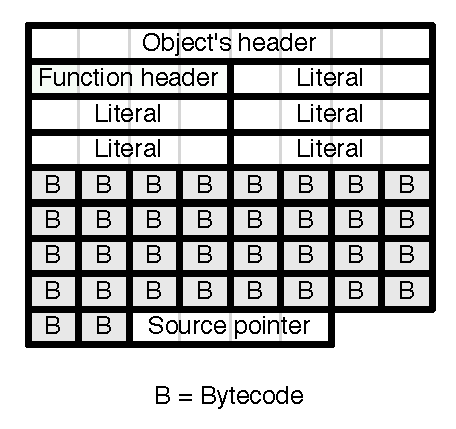
\includegraphics[width=0.4\linewidth]{CompiledCode}
        \caption{Virtual function representation}
        \label{fig:CompiledCode}
    \end{center}
\end{figure}

The bytecode set is stack-based. This means that most operations are pushing and popping values of the stack. All the operations are untyped and work with any object. One of the main instruction is the virtual call instruction, popping the receiver and arguments from the stack and pushing back the result. The bytecode set also includes conditional and unconditional branches to encode condition and loops, as well as specific bytecodes to create efficiently closures.


%Move to interface section I believe.

%+ complete list of bytecode instructions, maybe in appendix or a table ? Some of them are duplicated for interpreter performance and compaction (exemple, storePop and push nil), or more or less extended form (uncommon case tke more bytess) but does not really matter.

%Instr - meaning
%In meaning put in emph the variable (index, etc.)

%pushReceiver
%pushLit
%pushThisContext
%pop
%dup
%returnTop
%blockReturnTop

%*2
%pushTemp
%pushInstVar
%pushLitVar
%pushRemoteTemp

%send 
%superSend
%jumpOnTrue
%jumpOnFalse
%jumpForward
%jumpBackward

%createTempVect
%createClosure
%popIntoArray

\subparagraph{Virtual function installation.}

Classes and method dictionaries are normal objects in Pharo. Hence, the installation of a method uses normal dictionary APIs, inserted the selector and the method. Method dictionaries, upon modification, request the VM to flush look-up caches for the installed selector. As Pharo is dynamically typed and through uncommon behavior such as aggressive stack modification (modification of the receiver of the current frame) or primitives any method can be called by any object, flushing all the methods matching the selector is easier to implement and safer. Closure' functions are installed inside the method they are created in when the method is created, as a literal. Changing the literal (hence the closure's function) is normally not done in the current runtime.

\subparagraph{Primitive methods.}

Virtual methods can be annotated with a primitive number at creation time. A primitive method can be executed through a virtual call, like any other method, but upon activation a low-level function (either a Slang function or the native code generated from an assembly code template, depending on the current state of the runtime) is executed. The low-level code can fail if the receiver and arguments of the primitive method does not meet specific constraints. 

Although primitive methods can be used for performance, most of them provides essential features that could not be implemented otherwise. For example, the addition between two integers is implemented as a primitive, forwarding the operation to the processor's implementation of the addition.

Smalltalk features its set of exotic primitives, non present in most other programming languages. The best example is \ct{become:}, a primitive which swaps the references of two objects. If \ct{a become: b}, then all references to \ct{a} now refer to \ct{b}, and all the references to \ct{b} now refer to \ct{a}. This primitive is implemented efficiently based on Smalltalk specific strategies~\cite{Mir15a}.

The Sista architecture required the addition of a primitive method, detailled later in the thesis, and was using at some point exotic primitives such as \ct{become:}, until a better solution was found.

\paragraph{Registered objects.} An array of registered objects can be accessed in the Pharo runtime. This array contains multiple objects that need to be accessed by the VM, for example the objects \ct{nil, true} and \ct{false}. Any new object can be registered in the array, which can be requested to grow. 

Among registered objects are specific selectors. For example, the \ct{\#doesNotUnderstand:} selector is registered. When a look-up performed by the VM does not find any method to activate (the selector is not implemented for the given receiver), the VM instead performs a virtual call, using the same receiver, the registered \ct{\#doesNotUnderstand:} selector and reifies the virtual call as an object (which class is also registered) containing the original selector, the arguments and the look-up class in case of a super send. This strategy of registering a selector and using it in specific case to activate Smalltalk code is used in the Sista architecture to activate Scorch from the VM.

%%%%%%%%%%%%%%%%%%%%%%%%%%%%%%%%%%%%%%%%%%%%%%%%%%%%%%%%%%%%%%%%%%%%%%%%%%%%%%%%%%%%%%%%%%%%%%%%%%%%%%%%%%%%%%%%%%%%%%%%%%%%%%%

\section{Virtual machine}

The Pharo VM is a flavor of the Cog VM~\cite{Mira08a}. It relies on a v-function interpreter and Cogit to gain performance.

\subsection{Executable generation}

Most of the existing VM, inheriting from the original Squeak VM~\cite{Inga97a}, is written in Slang, a subset of Smalltalk. Slang is compiled to C and then to native code through standdard C compilers. The execution engine (the memory manager, the interpreter and the baseline JIT) are entirely written in Slang.

The slang code has two main advantages over plain C:
\begin{itemize}
	\item \emph{Specifying inlining and code duplication:} To keep the interpreter code efficient, one has to be very careful on what code is inlined in the main interpreter loop and what code is not. In addition, for performance, specific code may need to be duplicated. For example, the interpreter code to push a temporary variable on stack is duplicated 17 times, the 16 first versions are dedicated versions for temporary numbers 0 to 15, the most common cases, more efficient because of constant usage, and the 17th version is the generic version. Slang allows to annotate functions to direct Slang to C compilation, by duplicating or inlining specific functions. This feature is very important for uncommon processors where available C compilers are often less efficient to optimise C code.
	\item \emph{Simulation:} As Slang is a subset of Smalltalk, it can be executed as normal Smalltalk code. This is used to simulate the interpreter and garbage collector behavior. The JIT runtime is simulated using both Slang execution and external processor simulators. Simulation is very convenient to debug the VM as all the Smalltalk debugging tools are available. In addition, the simulator state can be saved and duplicated, which is very convenient to debug non deterministic garbage collection bugs.
\end{itemize}

The executable is generated in two steps. The first steps is to generate using the Slang-to-C compiler the two C files representing the whole execution engine written in Slang. Then, a C compiler is called and compiles the execution engine and additional C files (mostly the OS-specific code is written in C) to the executable VM.

\subsection{Baseline JIT}

Cogit is currently used as the baseline JIT. It takes a v-function as input, generates a n-function and installs it. Cogit performs three main kind of optimisations:
\begin{enumerate}
	\item \emph{Stack-to-register mapping:} As the v-functions are encoded using a stack-based bytecode set, values are constantly pushed and popped off the stack. To avoid this behavior, Cogit simulates the stack state during compilation. When reaching an instruction using values on stack, Cogit uses a dynamic template scheme to generate the native instructions. The simulated stack provides information such as which values are constants or already in registers. Based on this information, Cogit picks one of the available template for the instruction, use a linear scan algorithm to allocate registers that do not need to be fixed into a specific concrete register, and generate the native instructions.
	\item \emph{Inline caches:} Each virtual call is compiled to an unlinked inline cache. During execution, the inline cache is relinked to a monomorphic, polymorphic or megamorphic inline cache~\cite{Deut84a,Holz91a} when new receiver types are met. The inline caches improve performance but also allows, through n-function introspection, to determine which type is met for each virtual call site.
	\item \emph{Calling convention:} Cogit defines specific calling conventions for calls in-between n-functions. Typically, the receiver of the virtual call is always passed by register, and the arguments may or may not be passed by registers depending on how many there are. This is especially efficient to speed-up the inline cache logic and for primitive methods that have an assembly template available as they can directly use the values in registers.
\end{enumerate}

Cogit provides abstractions over the different memory managers supported by the VM (including 32-bits and 64-bits abstractions) and the different assembly back-ends. Most of the optimisations performed are platform-independent, through specific parts, such as inline cache relinking, needs to be implemented differently in each back-end. Cogit currently supports four different back-ends in production: x86, x64, ARMv6 and MIPSEL.

\subsection{Stack frame reification}

The VM intercepts all accesses to reified stack frames. The reified stack frame can be single, for example when created from Smalltalk and not by the VM, in which case it is a normal object and returning execution to it requires the VM to create a v-frame and marry it with the reified stack frame. In most cases, the reified stack frame is married and all accessed to it are intercepted, the VM then maps all the read and write operations to the current representation of the married frame (which is either a v-frame or a n-frame). Specific writes, typically the modification of the virtual instruction pointer or the caller, requires the frame to be divorced. The reified stack frame then becomes single, as if it was created from the Smalltalk, and returning execution to it requires the VM to create a v-frame and marry it. This kind of writes are unsafe and the Smalltalk program performing such operations needs to guarantee the operations won't lead to a crash, this is not the VM responsibility. 

Stack transformation (such as divorces) are handled by abusing stack page management. The stack is managed by the VM using multiple stack pages containing each between 40 and 60 frames on average. The VM uses different heuristic to ensure calls and returns across stack pages are uncommon in normal execution, as they are more expensive. Stack transformation usually split a stack page in two on the stack frame to modify, copying the lower part on another stack page. Returns across stack pages perform multiple checks, for example, returning to a single reified stack frame requires the creation of a v-frame and to marry them together.

%Maybe some figures, but which ones.

\ifx\wholebook\relax\else
    \end{document}
\fi